
\chapter{3D Heat Transfer Methodology}
\todo{reiterate why 3D simulations might be advantageous}

The methodology of the simulation begins with the validation case retrieved from \cite{ISO} is a 3D geometry consisting of the first and second floors separated by the floor slab and the plaster floor, the walls are aerated concrete, insulation, and brick. \todo{sentence doesn't sound right}
Below is a description of each component in the design software section and the roles of each software used \ref{fig:validation-case-materials} \textbf{(a)}.
\todo{below where?}


\todo{this transition makes no sense}
Then, we use Rhinoceros to create, export, and import geometries to create the mesh. 
\textit{Rhinoceros} will be used as a user interface to model the geometry and connect it to Grasshopper to calculate 3D heat transfer.
Grasshopper (GH) is a visual programming environment that we use to automate the OF simulation. Automation can find the coordinates of the points in the region to set the mesh, boundary conditions, and material properties. 
In addition, we use \textit{OpenFOAM}, which is an open source computational fluid dynamics (CFD) software package that is used to simulate fluid flow, heat transfer, and other capabilities. 


   
\begin{figure}[H]
     \centering
    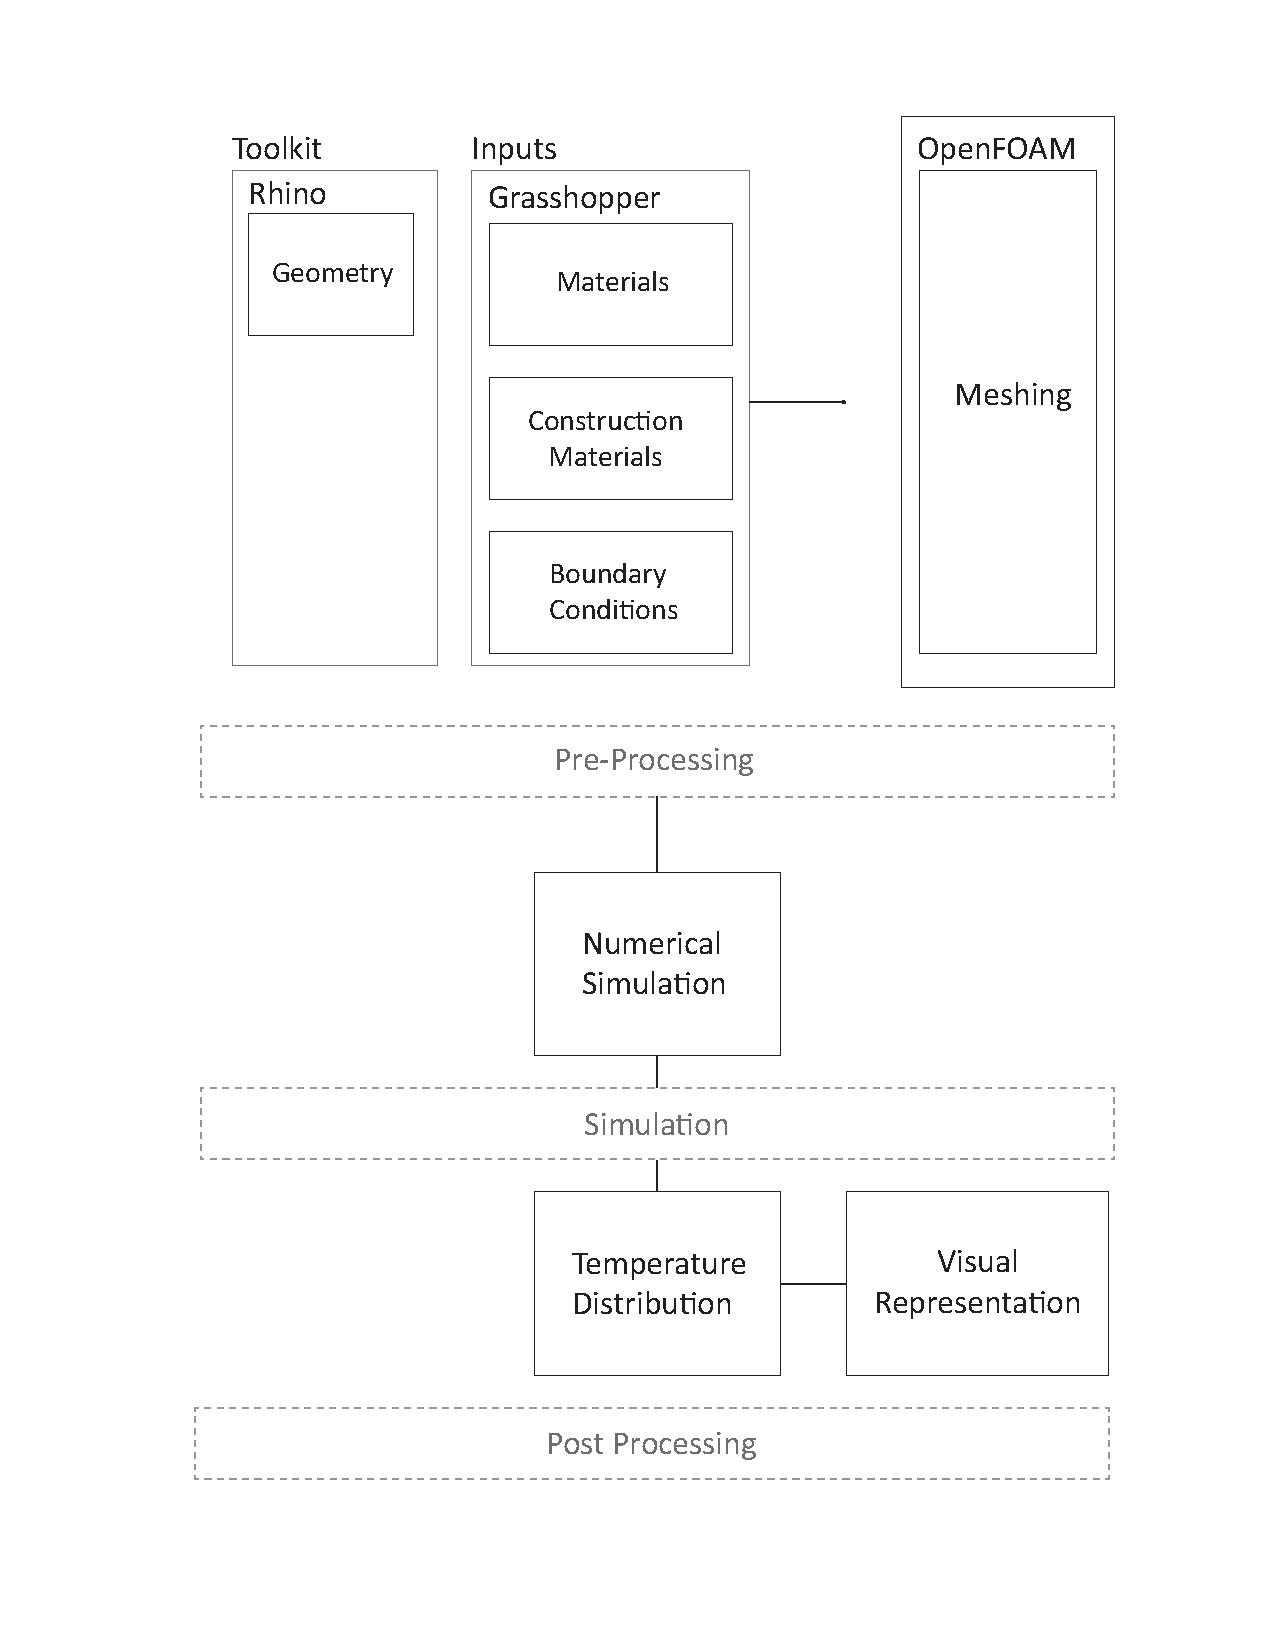
\includegraphics[trim=2.7cm 1.7cm 2.7cm 1.5cm, clip, width=0.7\linewidth]{Figures/flowchartv.pdf}
     \caption[Simulation Flowchart]{Flowchart of simulation steps starting from pre-processing to the post-processing of the simulation.}
   \label{fig:flowchart}
 \end{figure}


\section{Validation Case Study}
The case study used for this project is a validated 3D heat transfer case documented in \textit{ISO 10211:2007}\footnote{ISO 10211:2007---Thermal bridges in building construction. Validation of case A.3} \cite{ISO}. 
%One of the challenges we faced was retrieving this case study due to the lack of availability of validated 3D and not 2D heat transfer cases that incorporate building materials. 
Beyond \textit{ISO 10211:2007}, it is also documented in the \textit{QuickField} software where the properties, layers, and boundary conditions of the materials are accessible, which we exported to compare it with our method. 

   


\begin{figure}[H]
    \centering
    \begin{minipage}[t]{0.54\columnwidth}
        \centering
        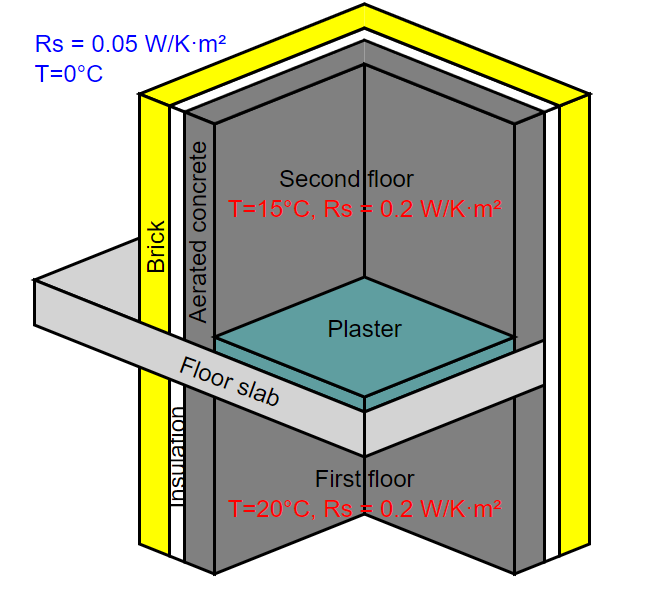
\includegraphics[width=\linewidth]{Figures/validationcase}
        \textbf{(a)}
    \end{minipage}
    \hfill
    \begin{minipage}[t]{0.8\linewidth}
        \centering
        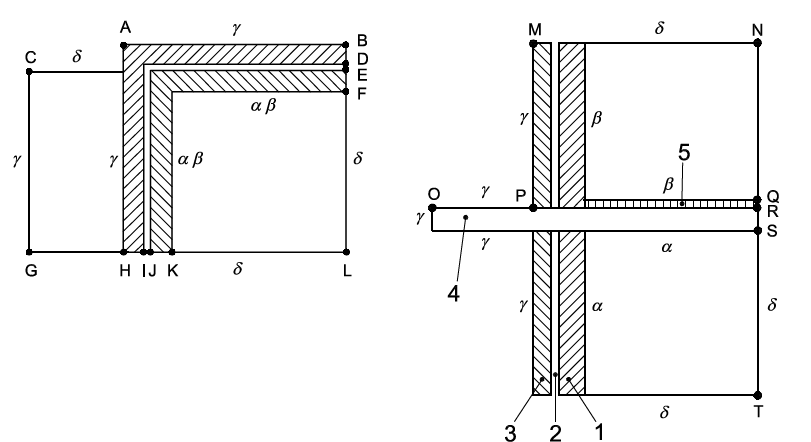
\includegraphics[width=\linewidth]{Figures/isodesc.png}
        \textbf{(b)}
    \end{minipage}
    
    \caption[3D Validation Materials]{Validation case materials \cite{ISO} \textbf{(a)} and Validation case sections retrieved from BS EN ISO 10211:2007(E) \textbf{(b)} \cite{ISO}.}
    \label{fig:validation-case-materials}
\end{figure}









\textit{QuickField}'s Heat Transfer module offers versatile features including steady-state or transient formulations with customizable initial field distributions and flexible time parameters, accommodating nonlinear specific heat and nonlinear or anisotropic properties. Although, the results include diverse thermal field mappings such as temperature, heat flux, and thermal gradients, editing and customizing the post-process options and locations were limited.



\begin{figure}[htb]
    \centering
    \begin{minipage}[t]{0.75\columnwidth}
        \centering
        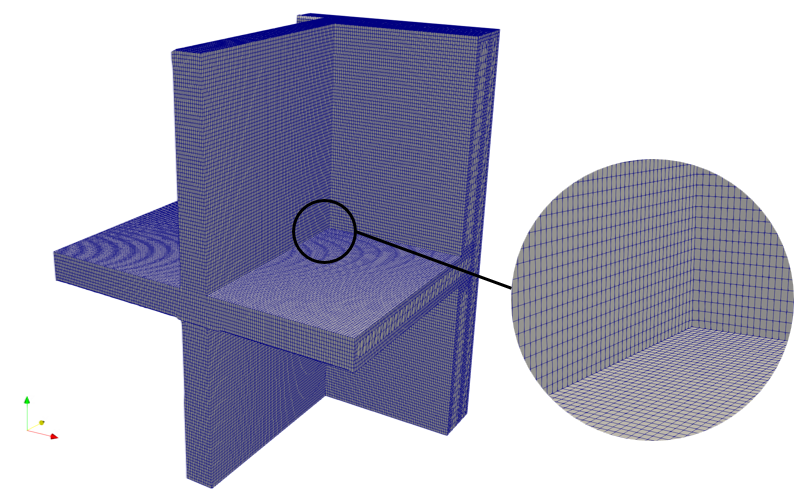
\includegraphics[width=\linewidth]{Figures/mesh3.png}
        \subcaption*{\textbf{(a)}}
    \end{minipage}
    \hfill
    \begin{minipage}[t]{0.5\columnwidth}
        \centering
        \begin{tabular}{clrrr}    
            \toprule
            & Type       & Multi-block dataset   \\ \midrule
            & \# of Cells & 360,364                      \\
            & \# of Points                        & 3,481,036                  \\
            & \# of TimeSteps                  & 400                        \\
            & Bounds X          & 0 to 1.9 (delta: 1.9) \\
            & Bounds Y          &                     0 to 1.25 (delta: 1.25) \\
            & Bounds Z          &                     -1 to 1.15 (delta: 2.15)    \\  \bottomrule
        \end{tabular}
        \caption*{\textbf{(b)} 3D Validation case mesh statistics.}
        \label{tab:mesh-stats}
    \end{minipage}
    
    \caption[3D Validation Mesh and Mesh Statistics]{\textbf{(a)} \textit{OpenFOAM} mesh viewed in $ParaView$ \textbf{(b)}  Validation case mesh statistics retrieved from BS EN ISO 10211:2007(E) \cite{ISO}.}
    \label{fig:validation-case}
\end{figure}




\section{Pre-processing}
The pre-processing phase consists of dividing the geometry into different zones based on different materials and locations. In addition, thermophysical properties, such as specific heat capacity and thermal conductivity, are assigned to materials, and fluid or solid properties are assigned to regions. Limit conditions and construction materials are specified in \cref{fig:validation-case-materials} \textbf{(a)} and \textbf{(b)}. 





\begin{table}[htb]
    \centering
    \label{tab:construction_material_properties}
    \caption[3D Material Properties]{Construction material properties and boundary conditions used for the simulation domain. Data were taken from the demo example in \textit{QuickField}.}
      \centering
        %\footnotesize
        \begin{tabular}{clrrr}    
            \toprule   
            & Materials       & $k$ $\left[ \si[per-mode=fraction]{\watt\per\metre\kelvin} \right]$ & $c_p$   $\left[ \si[per-mode=fraction]{\joule\per\kilogram\kelvin}\right]$ & $\rho$  $\left[ \si[per-mode=fraction]{\kilogram\per\cubic\metre} \right]$   \\
            \midrule
            & Floor Slab        & 2.5                        & 1000                      & 2300               \\
            & Aerated Concrete  & 2.5                        & 1000                      & 2300               \\
            & Brick             & 0.7                        & 1060                       & 710               \\
            & Insulation        & 1                         & 1450                      & 35               \\
            & Plaster           & 1                         & 1000                      & 2300              \\
            \bottomrule
        \end{tabular}
  
\end{table}


    \begin{table}[htb]
   
      \caption{3D Boundary Conditions}
      \centering
        %\footnotesize
        \begin{tabular}{llrr}    
            \toprule   
            & Boundary conditions          & $T [\si{\degreeCelsius}]$           & BC type                   \\ 
            \midrule
            & Inside temp.  (1st floor)         & 20                          & fixedValue                \\
            & Inside temp.  (2nd floor)          & 15                          & fixedValue                \\
            & Outside temp.  & 0                          & fixedValue                \\ 
            \bottomrule
        \end{tabular}

\end{table}






\subsubsection{Case Study setup}
The case study geometry was exported from \textit{QuickField} and then modeled in \textit{Rhinoceros} and subsequently exported as a mesh to be processed with OpenFOAM where \ref{meshsteps} visualizes the steps to create the mesh. 
The validation case was constructed in \textit{OpenFOAM} by creating the mesh and \textit{snappyHexMesh} files.  
\ref{fig:validation-case-materials}  (b) illustrates the \textit{OpenFOAM} mesh visualized in \textit{ParaView}.
    

\begin{figure}[htb]
     \centering
    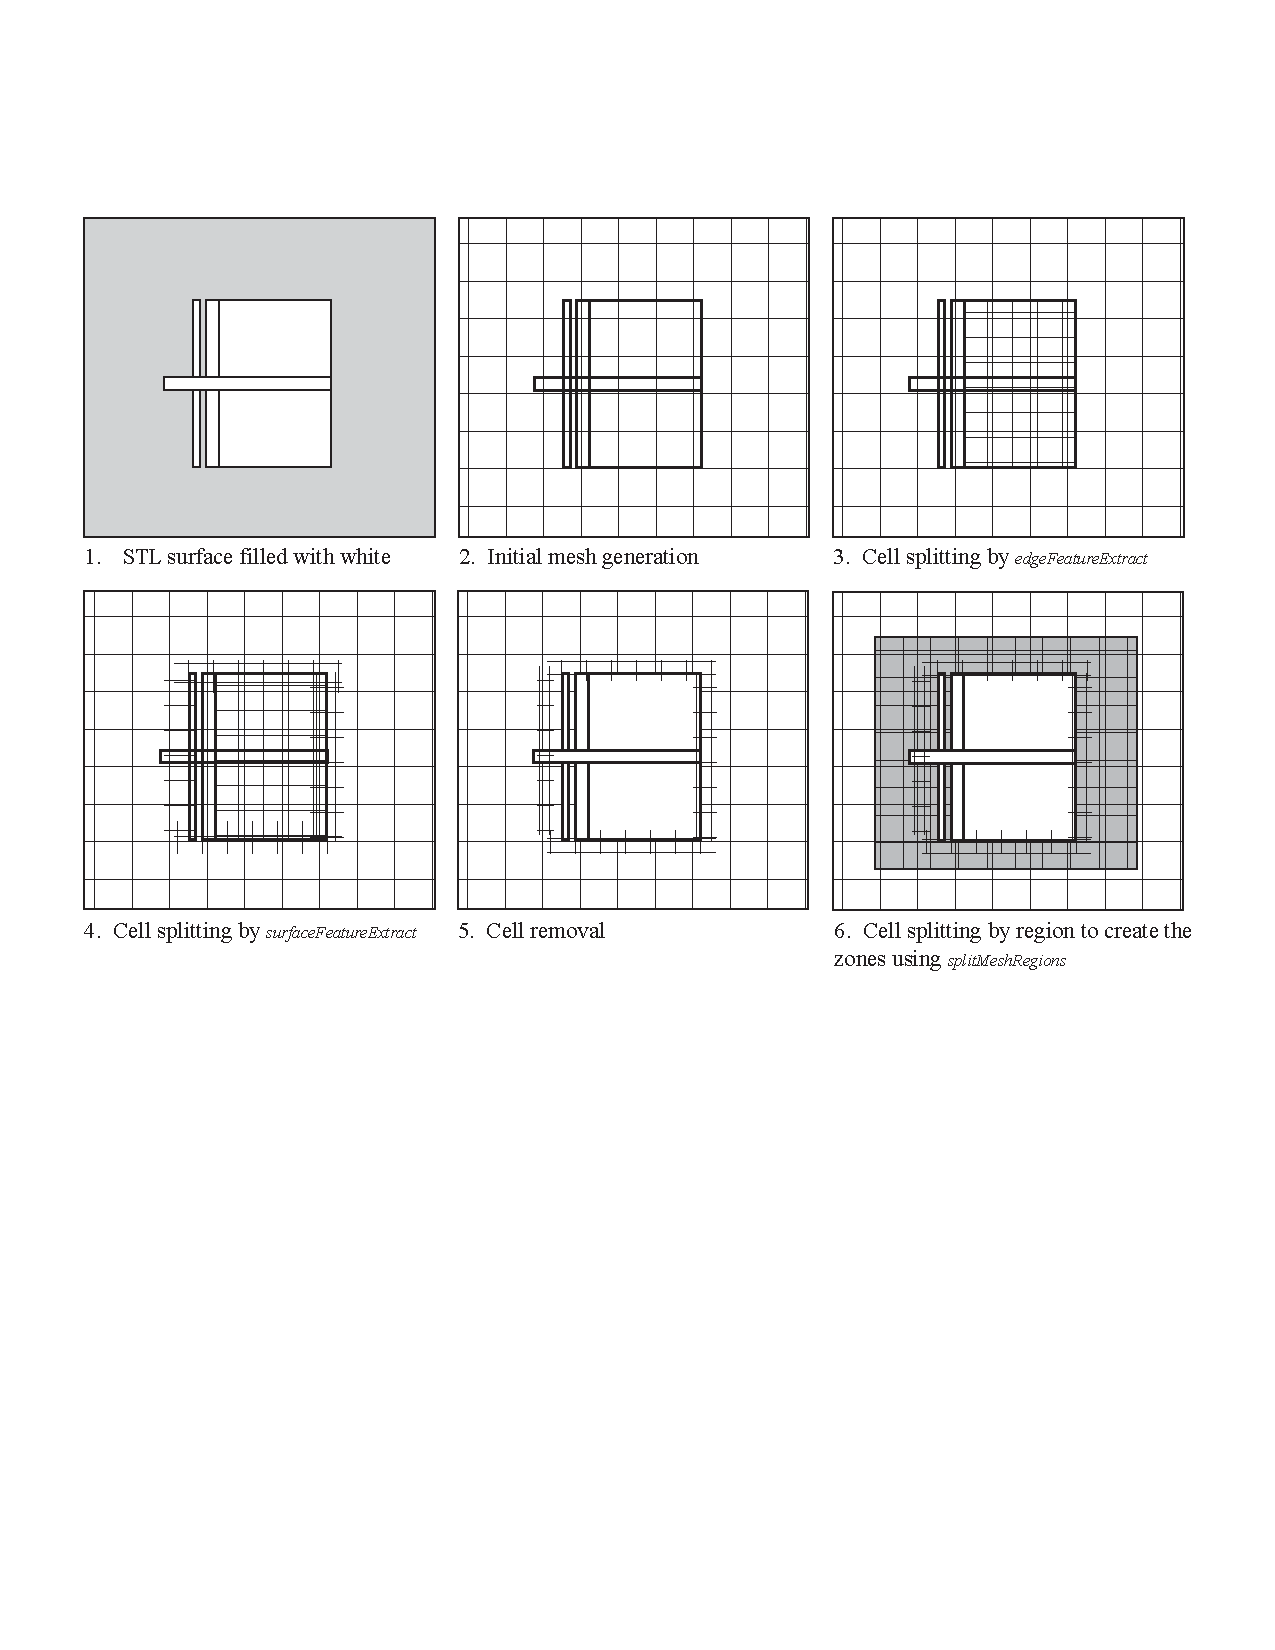
\includegraphics[trim=1cm 11cm 1cm 3cm, clip, width=0.9\linewidth]{Figures/snappyhex.pdf}
     \caption[Mesh Creation Steps]{Visualization of the steps and executables to create the mesh step-by-step}
   \label{meshsteps}
   \todo{nice figure, but I am not sure it shows what is happening. Aren't we cutting the cells outside of the geometry, leaving the inside? This is the opposite of what Eddy3D does.}
 \end{figure}


%\clearpage
\section{Simulation Equations}

\subsection{Solver Setup}
The solver used in this case is \textit{chtMultiRegionFoam} in OpenFOAM 2306 which is a solver capable of solving for steady or transient fluid flow with solid heat conduction and conjugate heat transfer between regions, buoyancy effects, turbulence, reactions, and radiation modeling\footnote{Not used in this study.} \cite{cht}.
There are three solvers capable of simulating steady-state heat transfer between fluids and solids which are \textit{chtMultiRegionFoam}, \textit{chtMultiRegionSimpleFoam}, and \textit{chtMultiRegionTwoPhaseEulerFoam}, but, the main difference is that the selected solver for this case is capable of doing both steady and transient states to have a more sufficient software. 
\todo{more sufficient software?}

To precisely mimic real-world situations, The use of \textit{chtMultiRegionFoam} solver is essential to have accurate 3D heat transfer results due to the availability of using fluid and solid. \ref{interface} visualizes the capabilities of the solver with the various domains and interfaces of different temperatures, solids, and fluids. 
A description of the boundary conditions can be found in \cref{{tab:construction_material_properties}}. 
However, the outdoor temperature is set to be 0 degrees Celsius and climate Setup can be easier by using Grasshopper to leverage the initial temperatures based on the location. 
Another crucial aspect is identifying the thermal properties that will allow the solver to identify the thermal conductivity, density, and properties of the material and calculate the heat transfer accordingly.


\subsection{Physical models}
The physical models found in the constant file are required for the simulation to run according to the OpenFOAM documentation \cite{OFD}.

\subsubsection{Turbulence Properties}
The turbulence used for steady-state heat transfer is Reynolds Averaged Simulation (RAS), where the full form is anisotropic contribution of the Reynolds stress is shown below to influence the motion of a fluid, providing a comprehensive understanding of fluid flow dynamics. Where the heat conservation equation according to \cite{hce}

\begin{equation}
u_i \frac{\partial T}{\partial x_i} + \frac{\partial}{\partial x_i}(K_T \frac{\partial T}{\partial x_i}) = 0 \label{eq:heat}
\end{equation}

where $u_i$ is the velocity component in the i-direction, T is the temperature, $x_i$ is the spatial coordinate in the i-direction, $K_T$ is the thermal conductivity coefficient.


Then the Navier-Stokes equation, which describes the conservation of momentum for a fluid:
\begin{equation}
\frac{\partial (\rho {u}i)}{\partial t} + \frac{\partial}{\partial x_j} \left( \rho {u}i u_j \right) = -\frac{\partial p}{\partial x_i} + \frac{\partial}{\partial x_j} \left( \tau{ij} + \tau{t_{ij}} \right) + \rho g_i
\end{equation}




Where, $\rho$ is the density of the fluid, $u_i$ is the velocity component in the $i$-direction, $t$ is time, $x_i$ is the spatial coordinate in the $i$-direction, $p$ represents pressure, $\tau_{ij}$ is the viscous stress tensor, $\tau_{t_{ij}}$ is the turbulent stress tensor, and $g_i$ is the gravitational acceleration in the $i$-direction
 \cite{cht}.


\subsubsection{Thermophysical Models}
The thermophysical properties located in each zone and the constant file require inputs of density $\rho$, thermal conductivity, and specific heat capacity for every material.
\subsubsection{Finite Volume Options}
The fvOptions text file allows the user to further manipulate the systems of equations, such as sources and skins. 

\subsection{Solver Equations}    
\todo{are these the equations that CHT is based on? If yes, then say so.}
This section presents the implementation of heat transfer equations and metrics into OpenFOAM and the solver from OpenFOAM Foundations\cite{OpenFOAMFoundation}
\subsubsection{Fluid Equations}

      Mass Conservation is \begin{equation}
\frac{\partial \rho}{\partial t} + \frac{\partial (\rho u_j)}{\partial x_j} = 0
\end{equation}


      Momentum Conservation Equation is \begin{equation}
\frac{\partial (\rho u_i)}{\partial t} + \frac{\partial}{\partial x_j} \left( \rho u_{rj} u_i \right)  + \rho\epsilon_{ijk}\omega_i u_j = - \frac{\partial p_{rgh}}{\partial x_i} - \frac{\partial \rho g_j x_j}{\partial x_i}  + \frac{\partial}{\partial x_j} \left( \tau_{ij} + \tau_{t_{ij}} \right)
\end{equation}
\todo{you already have a similar for of the NS equation above in the turbulence section}


\subsubsection{Solid Equations}
Solid Energy Conservation is \begin{equation}
\frac{\partial (\rho h)}{\partial t} = \frac{\partial}{\partial x_j}\left( \alpha \frac{\partial h}{\partial x_j} \right)
\end{equation}

where \( h \) is the specific enthalpy, \( \rho \) is the density, and \( \alpha = \frac{\kappa}{c_p} \) is the thermal diffusivity, and the specific heat capacity \( c_p \). 


\subsubsection{Solid and Fluid Interface}
\begin{equation}
T_f = T_s  \\
Q_f = -Q_s  \\
\kappa_f \frac{d T_f}{d n} = -\kappa_s \frac{d T_s}{d n} 
\end{equation}

where \( \kappa_f \) thermal conductivity of the fluid and \( \kappa_s \)  the thermal conductivity of the solid.


\subsection{Constructing The Case}    
An OF steady state heat transfer case requires three main folders to run which are iteration \textit{0}, \textit{constant}, and \textit{system} folders. Each folder is responsible for properties or boundary conditions and includes these conditions in each zone in the geometry. The 10 zones in the case which are \textit{Brick}, \textit{Slab}, \textit{Plaster}, \textit{ConreteTop}, \textit{ConreteBottom}, \textit{IntAirTop}, \textit{ExtAir}, \textit{IntAirBottom}, \textit{InsulationTop}, and \textit{InsulationBottom}. Below in \cref{constc} is an explanation of the case contents. The text files in this case are written automatically due to the script setup in GH. While constructing the constant file, the specific heat capacity of each material was needed, so we followed the steps below to find it (Brick Example):

\begin{equation}
\begin{aligned}
\Delta T &= 15^\circ \text{C} \\
d &= 100 \, \text{mm} = 0.1 \, \text{m} \\
A &= 1300 \times (950 + 50 + 50 + 950) \, \text{mm}^2 \\
A &= 1300 \times (2000) \, \text{mm}^2 = 2.6 \, \text{m}^2 \\
Q &= \frac{k \cdot A \cdot \Delta T}{d} \\
&\text{solve for the specific heat capacity ($C_p$):} \\
C_p &= \frac{Q \cdot d}{k \cdot A \cdot \Delta T} \\
Q &= k \cdot A \cdot \frac{\Delta T}{d} \\
Q &= 0.7 \, \text{W/m.K} \times 2.6 \, \text{m}^2 \times 15^\circ \text{C} / 0.1 \, \text{m} \\
Q &= 27 \, \text{W} \\
C_p &= \frac{27 \, \text{W} \times 0.1 \, \text{m}}{0.7 \, \text{W/m.K} \times 2.6 \, \text{m}^2 \times 15^\circ \text{C}} \\
C_p &= \frac{2.7 \, \text{J}}{2.55 \, \text{J/K}} \\
C_p &\approx 1.06 \, \text{kJ/kg.K} \\
&\text{So, the specific heat capacity of the brick is approximately} \, 1.06 \, \text{kJ/kg.K} \\
&\text{To convert to J/kg.K:} \\
C_p &= 1.06 \, \text{kJ/kg.K} \times 1000 \\
C_p &= 1060 \, \text{J/kg.K}
\end{aligned}
\end{equation}
\todo{add this to the appendix and refer to it in the text.}







\begin{figure}[H]
\centering
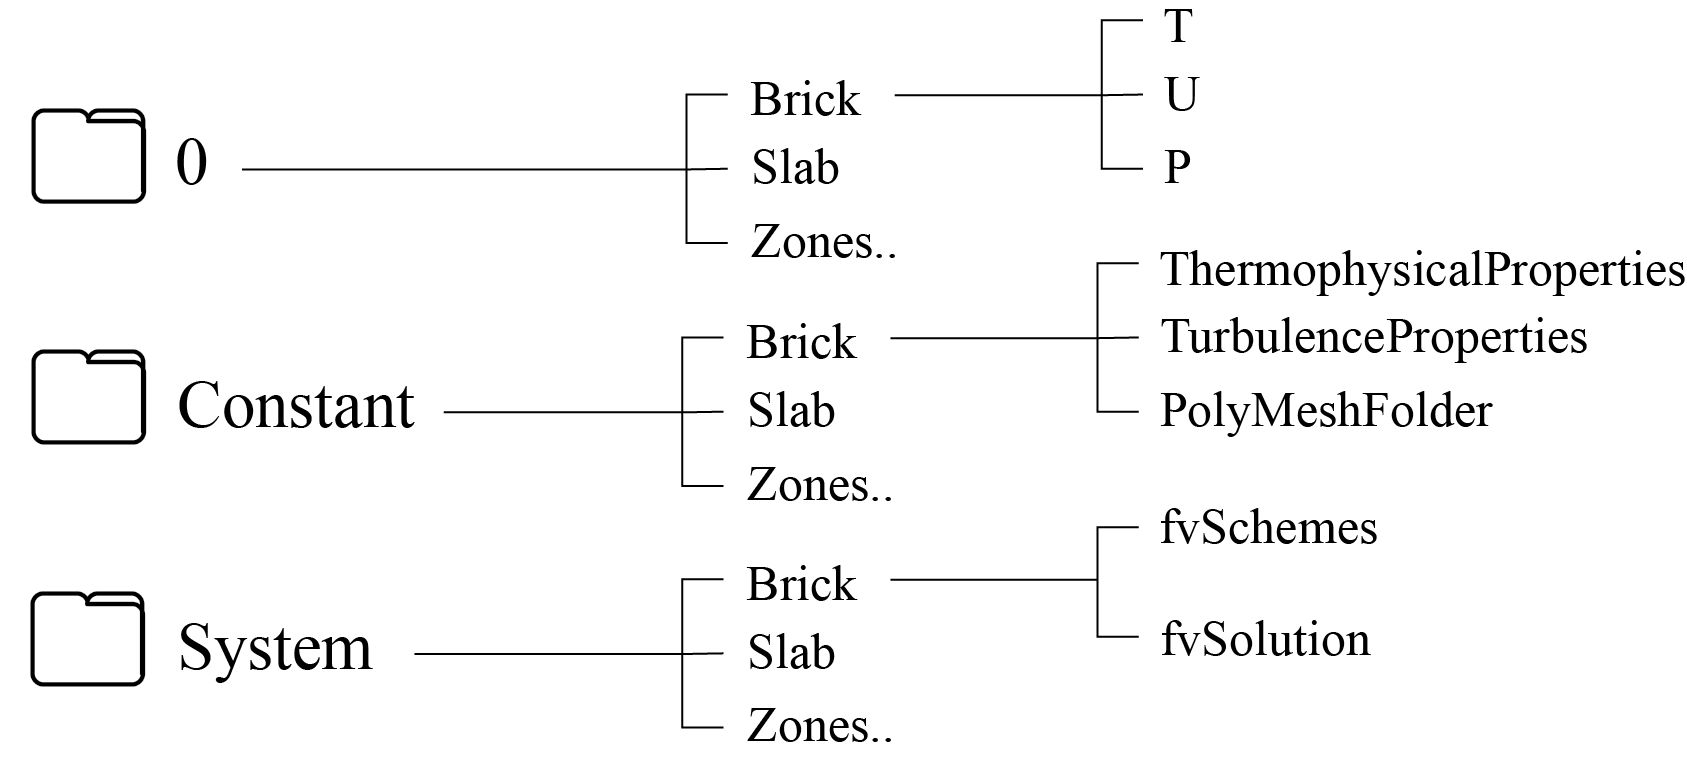
\includegraphics[width=0.77\columnwidth]{Figures/constc.png}
\hspace{0.7cm}
\caption[OF Case Contents]{OF case folders to run. Where (zones..) represent a folder for each zone in the case.}
\label{constc}
\end{figure}


\subsection{OF Text files Automation by GH}   
This section explains the Grasshopper script that automatically creates and exports STL files, defines material properties, finds the point location in the meshes, and writes all the text files needed to run the OF case.

\subsubsection{Materials Properties Component}
The component shown in \ref{matgh} is a dictionary for the material connected to specific geometry. Each different zone in Rhino needs to be connected to the shown component by adding the corresponding specifications for the material such as the name, type, temperature, specific heat capacity, thermal conductivity, and density. This component is considered the base and many other sections in the script depend on it such as writing the other text files in 0 files where the boundary conditions are needed or writing the constant and system files. 


\begin{figure}[H]
\centering
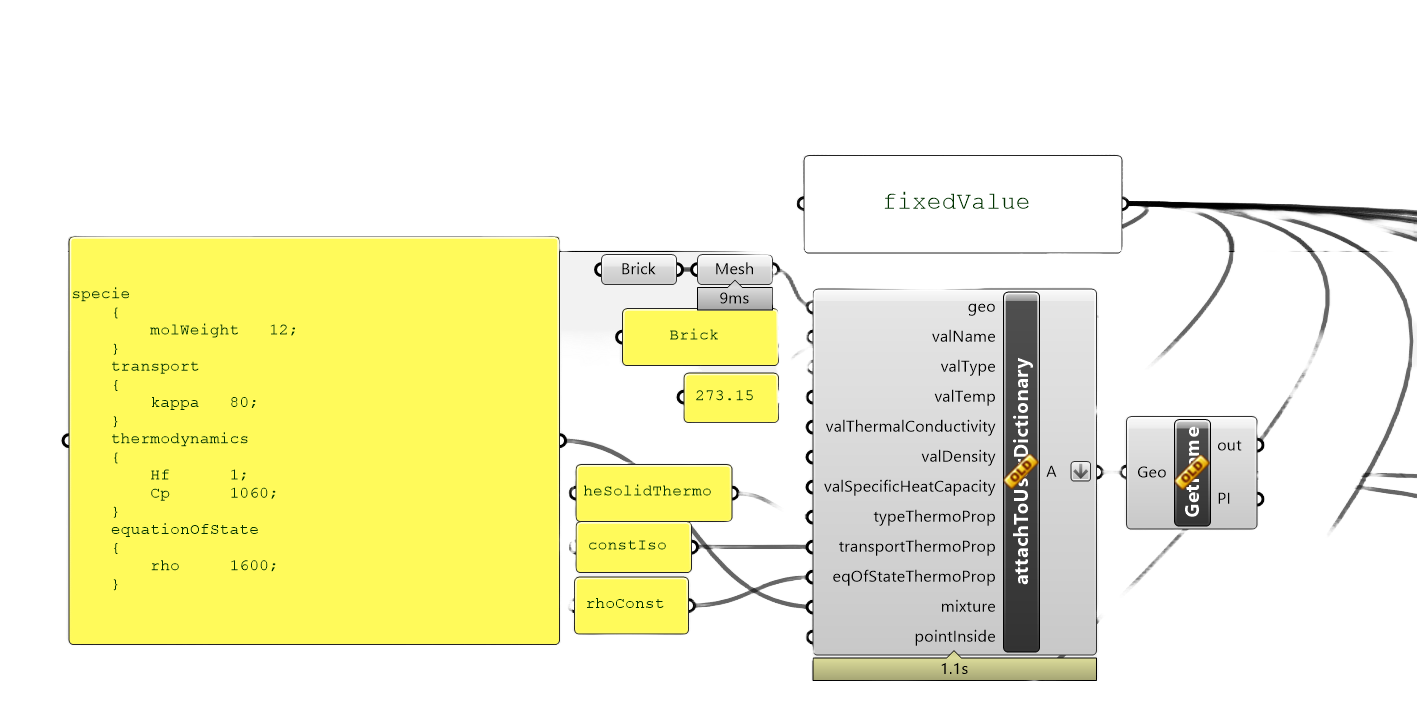
\includegraphics[width=0.77\columnwidth]{Figures/materialgh.png}
\hspace{0.7cm}
\caption{GH Material Properties Component}
\label{matgh}
\end{figure}



\subsubsection{STL Files to Create the Mesh}
The workflow shown in \ref{stlgh} is used to create an STL from the geometry in Rhino and export it to the \textit{trisurface} in the constant file to create the mesh using the mesh generation utility, \textit{snappyHexMesh} where an explanation is in \ref{meshsteps}.


\begin{figure}[H]
\centering
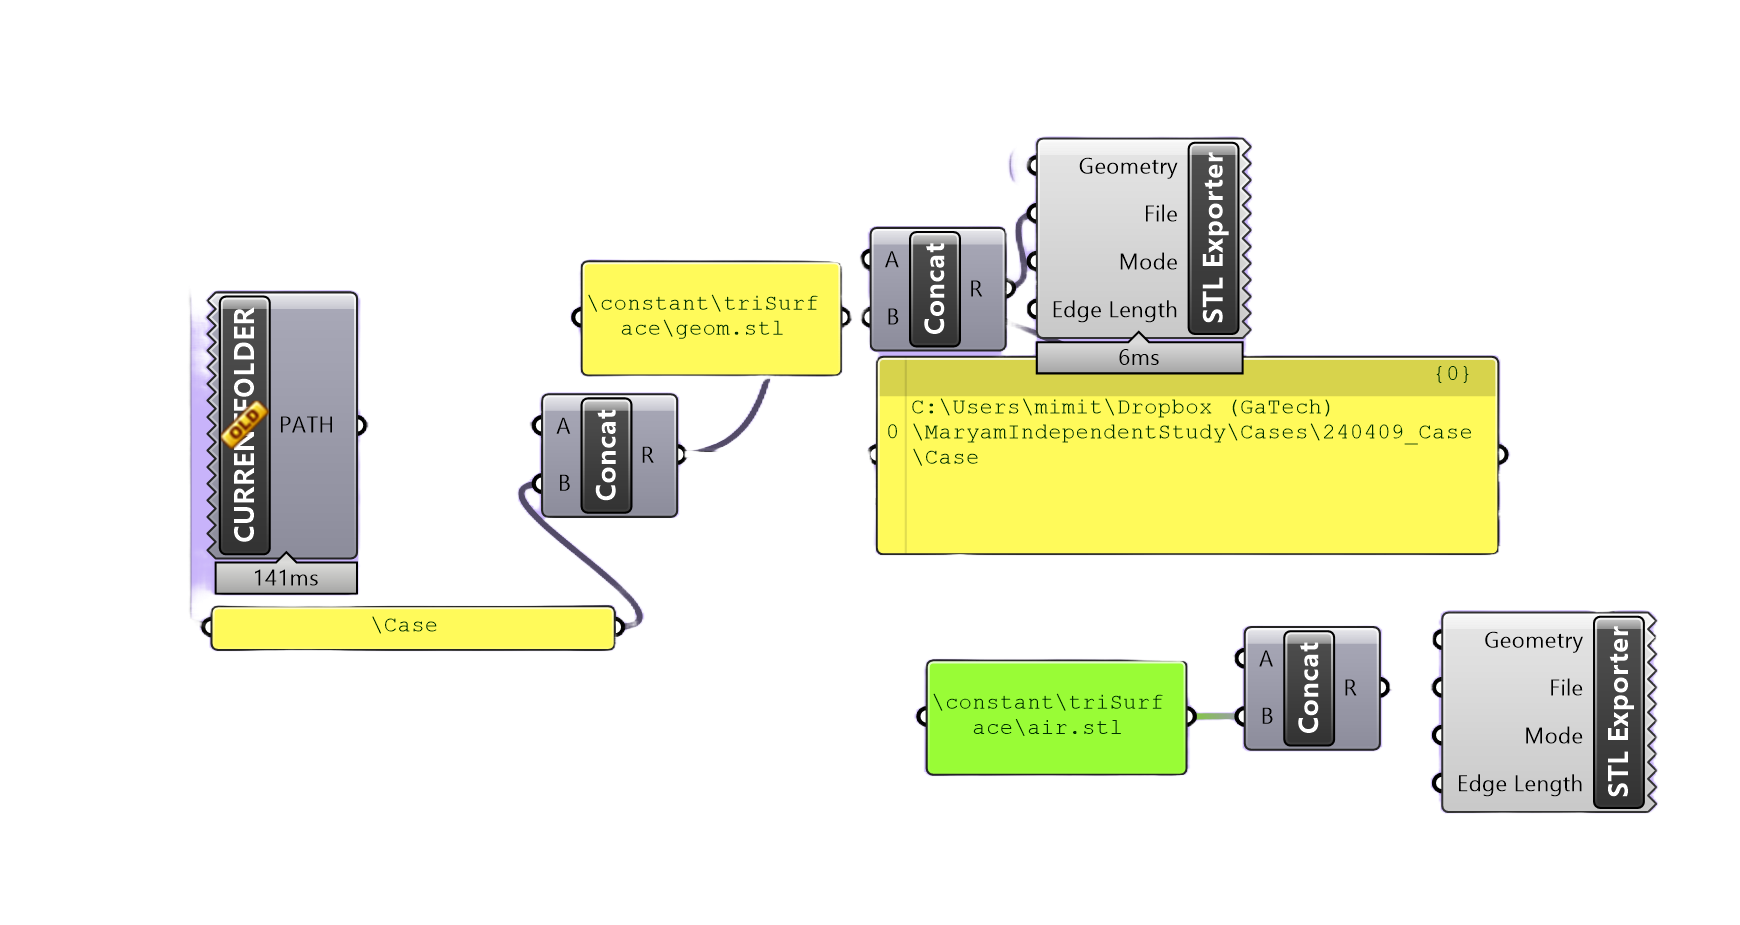
\includegraphics[width=0.77\columnwidth]{Figures/stlgh.png}
\hspace{0.7cm}
\caption{GH STL Workflow}
\label{stlgh}
\end{figure}
\todo{this figure is not useful}



\subsubsection{GH Point in Mesh}
The workflow in \ref{locgh} automatically defines the point coordinates of each region in the mesh. Each region must have a point in Rhino and the points each are connected to the corresponding material component. The \textit{locationInMesh} parameter identifies a specific point within the computational domain, allowing the \textit{snappyHexMesh} tool to identify and locate all cells that are connected to that point. This helps ensure that only certain regions/zones are kept during the mesh generation process, usually to separate different volumes or regions of interest.

In our case, one point is not enough to capture all the 10 regions, so, using the \textit{locationsInMesh} is essential. This allowed us to specify a list of points that represent various locations within the mesh. Each point in this list creates a separate cell zone located in the constant/ConcreteTop/polyMesh/cellZones file, allowing more complex meshing and region differentiation. This flexibility is useful for our case and other complex geometries within a single mesh.

\begin{figure}[tbh]
\centering
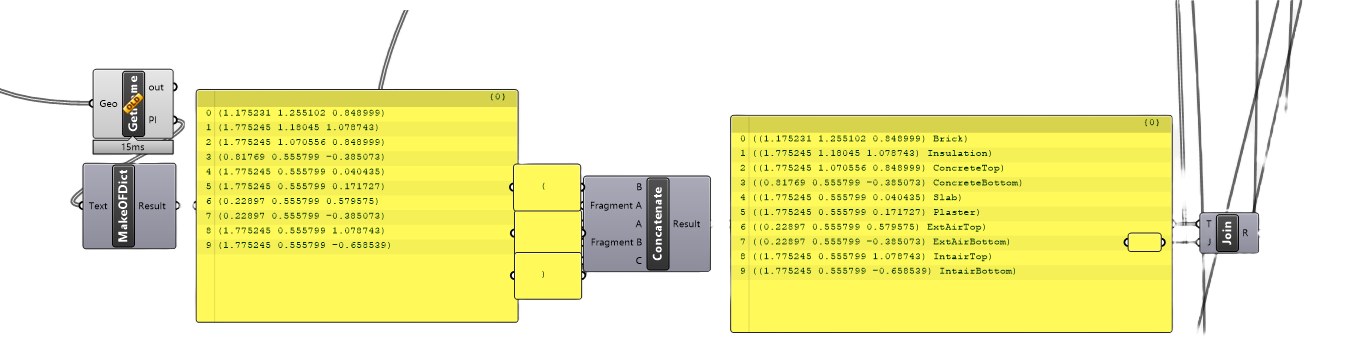
\includegraphics[width=0.77\columnwidth]{Figures/locinmeshgh.png}
\hspace{0.7cm}
\caption{GH Point in Mesh Workflow}
\label{locgh}
\end{figure}





\subsubsection{Block Mesh Boundary}
\ref{blkmgh} includes a component similar to the materials component but is responsible for automatically writing the boundary conditions of minx,maxx,miny,maxy,minz, and maxz. 

\begin{figure}[tbh]
\centering
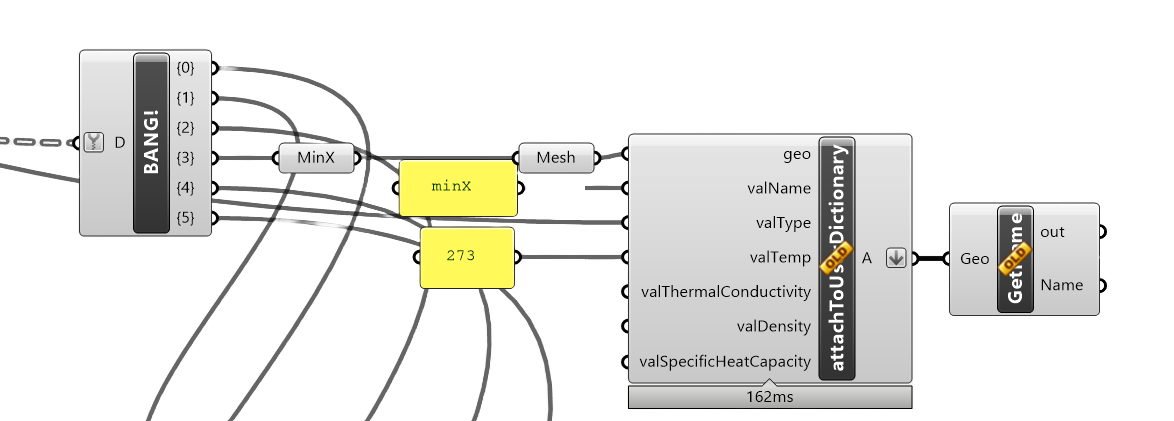
\includegraphics[width=0.77\columnwidth]{Figures/bcondgh.png}
\hspace{0.7cm}
\caption{GH Boundary Conditions Component}
\label{blkmgh}
\end{figure}




\subsubsection{Surface Combinations}
The surface combinations workflow shown in \ref{surfgh} writes the zones interfaces to be used in each zone text file in constant, system, and 0. 

\begin{figure}[tbh]
\centering
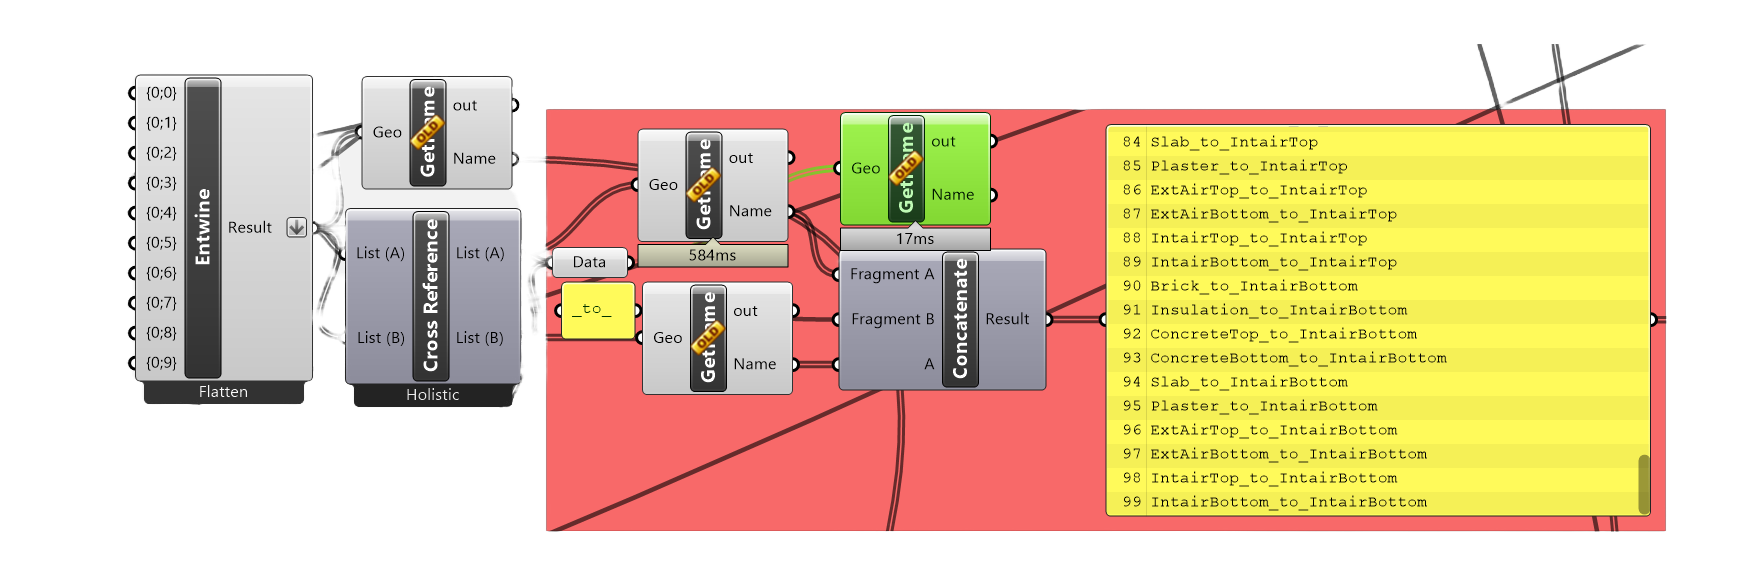
\includegraphics[width=0.77\columnwidth]{Figures/intergh.png}
\hspace{0.7cm}
\caption{GH Surface Combinations Workflow}
\label{surfgh}
\end{figure}
\todo{I would not show screenshots of your script if you keep it so disorganized.}


\subsubsection{Write P File Example}
The sample in \ref{Pgh} writes all of the P files needed to run the simulation for each zone. All of the other required text files such as T and U are written using the same workflow where the component includes a script that writes the text file in the OF required format. Also, all of the needed boundary conditions and material specifications are taken from the material dictionary component in \ref{matgh}.


\begin{figure}[tbh]
\centering
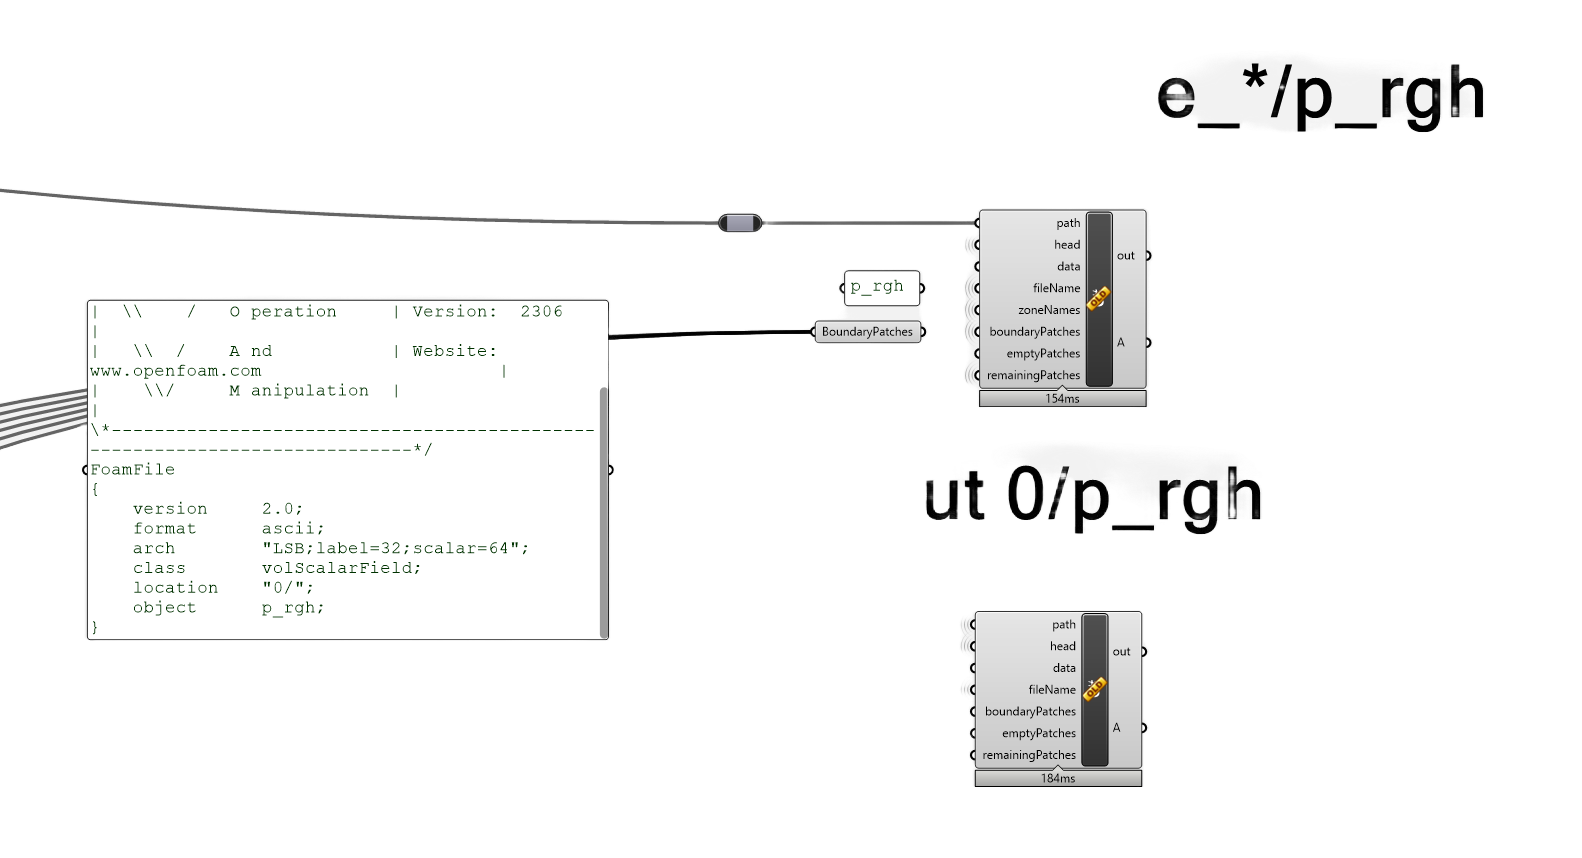
\includegraphics[width=0.77\columnwidth]{Figures/writepgh.png}
\hspace{0.7cm}
\caption{GH Write P File Workflow}
\label{Pgh}
\end{figure}
\todo{this figure is not useful}


















\subsection{Running The Case}    
 
After discussing the selected solver capabilities to run the numerical simulation. The goal is to solve heat transfer in solid and liquid regions between air regions and the selected geometry. Using the software \textit{QuickField}  to solve for 3D heat transfer showed some limitations where it does not consider the air regions. However, our approach using OpenFOAM includes the integration between air and solids to produce more accurate results. 

\begin{figure}[tbh] 
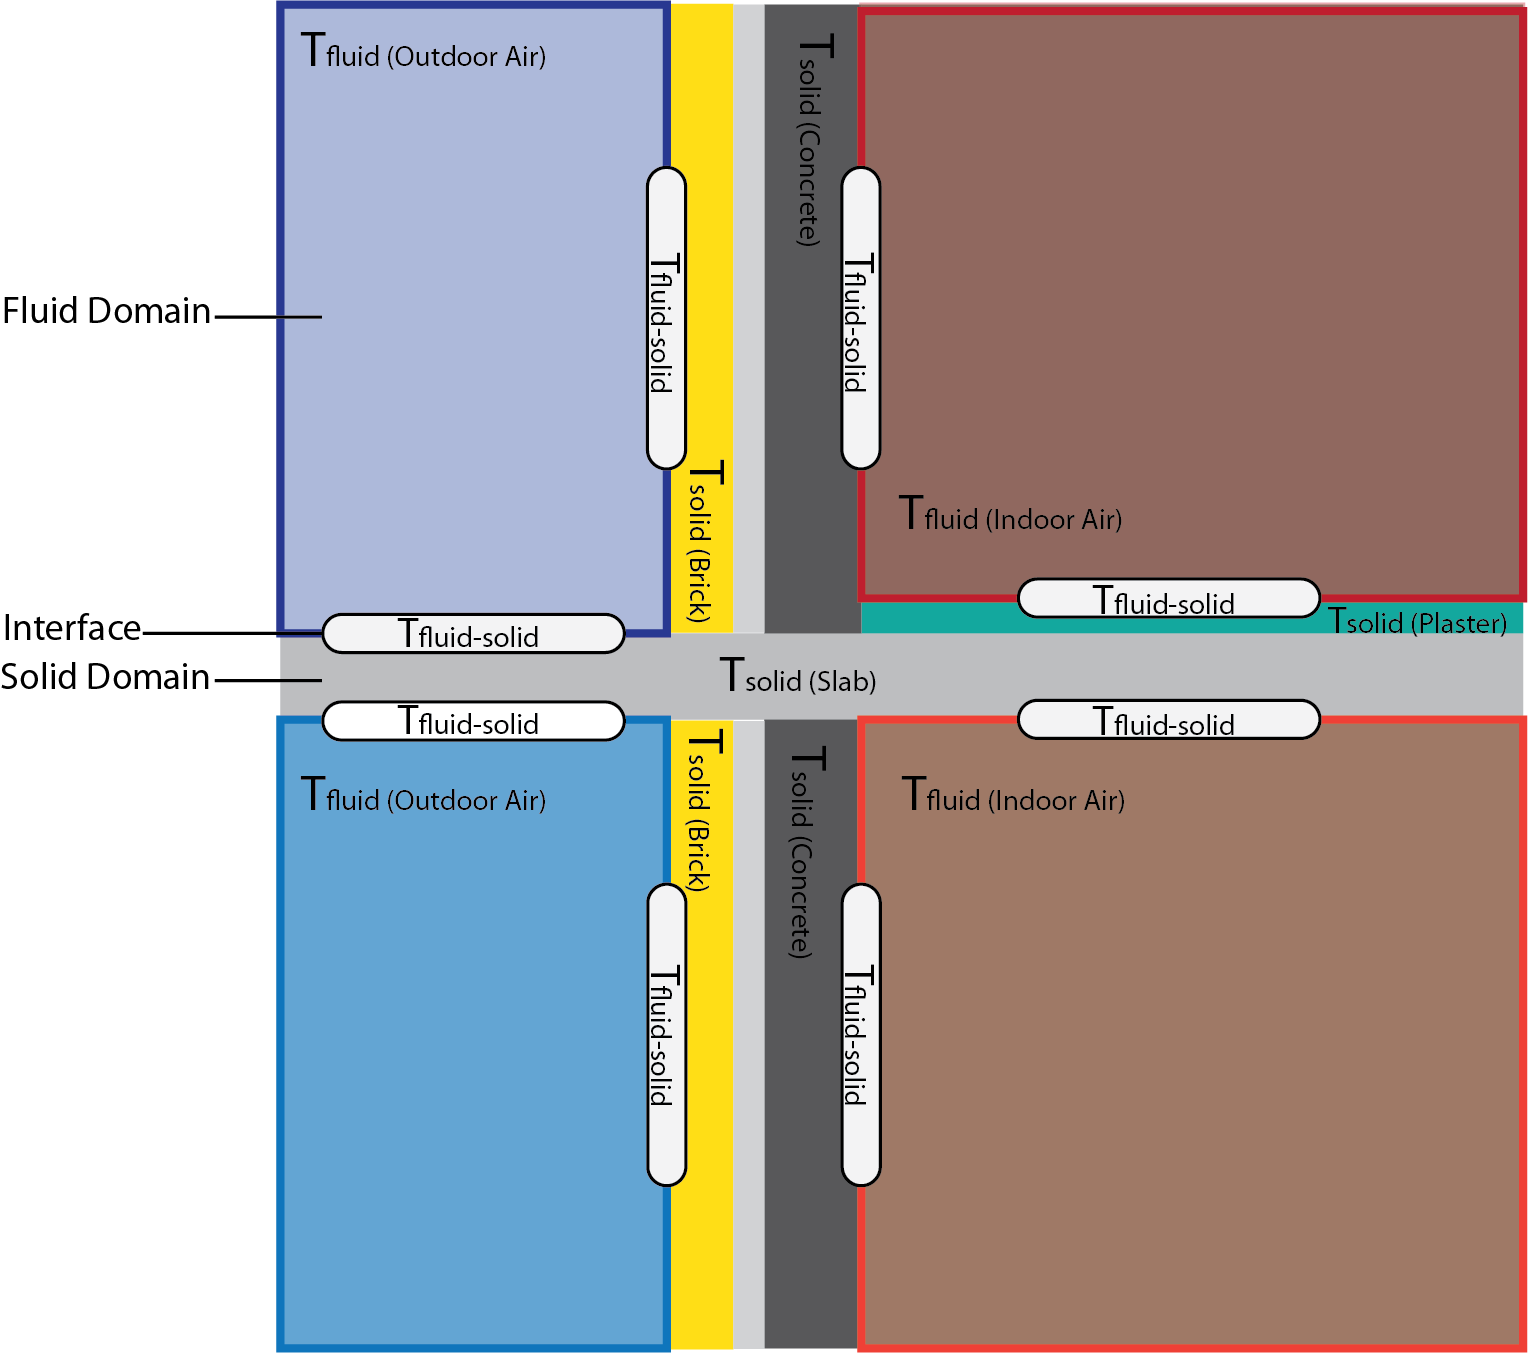
\includegraphics[width=0.77\columnwidth]{Figures/conductive.png}
\hspace{0.7cm}
\caption[3D Interfaces]{Vertical section of the validation case shows convection and conduction.}
\label{interface}
\end{figure}

\begin{figure}[tbh]
\centering
\begin{tikzpicture}[node distance=1.85cm, thick, every node/.style={scale=1}]
% Define nodes
\footnotesize
\node (blockMesh) [block] {blockMesh};
\node (surfaceFeatureExtract) [block, below of=blockMesh] {surfaceFeatureExtract};
\node (snappyHexMesh) [block, below of=surfaceFeatureExtract] {snappyHexMesh};
\node (splitMeshRegions) [block, below of=snappyHexMesh] {splitMeshRegions};
\node (chtMultiRegionFoam) [block, below of=splitMeshRegions] {chtMultiRegionFoam};
% Connect nodes with arrows
\draw [arrow] (blockMesh) -- (surfaceFeatureExtract);
\draw [arrow] (surfaceFeatureExtract) -- (snappyHexMesh);
\draw [arrow] (snappyHexMesh) -- (splitMeshRegions);
\draw [arrow] (splitMeshRegions) -- (chtMultiRegionFoam);
\end{tikzpicture}

\caption[OF Executable]{Order of executables for multiregion case setup with OpenFOAM v2306.}
\label{fig:order-of-executables}
\end{figure}






\ref{fig:order-of-executables} illustrates the executables that need to be executed in order for a multi-region case.
The \textit{blockMesh} utility generates parametric meshes incorporating grading and curved edges. 
The meshes are created based on the specifications outlined in a dictionary file named \textit{blockMeshDict}  within the case directory.
\textit{surfaceFeatureExtract} extracts the surface features and then records them in a file.      
\textit{snappyHexMesh} is a utility in OpenFOAM that generates 3D meshes with hexahedra from STL surfaces, iteratively refining while maintaining surface conformity.
\textit{splitMeshRegions} divides the mesh into separate regions. Each region consists of cells reachable without crossing boundary faces, including cell zones.
\textit{chtMultiRegionFoam} is a solver for both steady and transient fluid flow, with solid heat conduction and conjugate heat transfer. The equations for each system variable are solved, and the solutions from the preceding equations are inserted into the subsequent ones. For instance, fluid-solid coupling solves fluid equations first, using the previous iteration's solid temperature to set fluid temperature boundary conditions. Then we solved the fluid equations using the same method. The simulation using this process continued until convergence at time step 400.
    



%\clearpage
\section{Post-processing}
The post-processing section consists of two methods to visualize the data. The first method is using \textit{Paraview} to visualize the outcome and process the results. The second method is \textit{OpenFOAM}'s post-process command, first, select the probing locations using GH automation components to automatically write the post-processing file and measure the data, then plot the data to compare the validation case temperatures with our results. 

(WRITE HOW YOU DID POST PROCESSING AND ADD IMAGES)


\section{Results}
This section discusses the results of key experimental results of our ongoing research. 
\cref{fig:validation-plots} \textbf{(a)} visualizes the simulation temperature output, including the air (fluid) regions. Whereas
\cref{fig:validation-plots} \textbf{(b)} shows the geometry excluding the air, which represents the temperature distributions. The resulting temperatures are shown in the plot in \cref{fig:validation-plots}. The plot includes the \textit{QuickField} outputs and our OpenFOAM simulation along the z-axis from $z= 1.2$ to $z=2.2$ (the red line shown in \cref{fig:validation-plots} \textbf{(a)}) and represents non-linear progression as a result of the different specific heat capacities and thermal conductivity of the materials. The peak in z=1.8 refers to the temperature of the slab, where it can be modified by readjusting the slab model and re-simulate. 



\begin{figure}[tbh]
    \centering
    \textbf{a}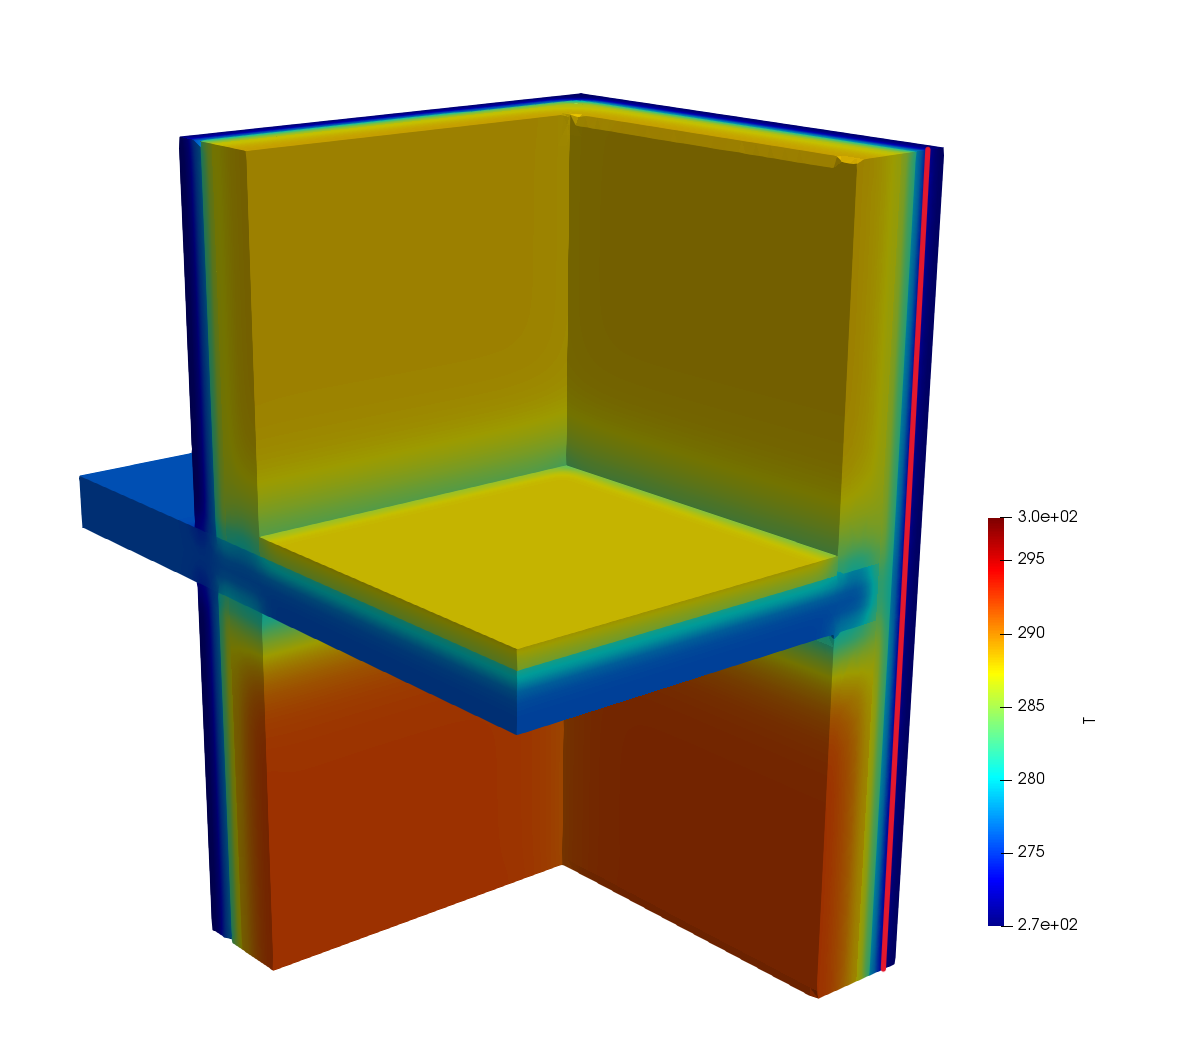
\includegraphics[width=0.65\columnwidth]{Figures/casewoutair.png}
    \textbf{b}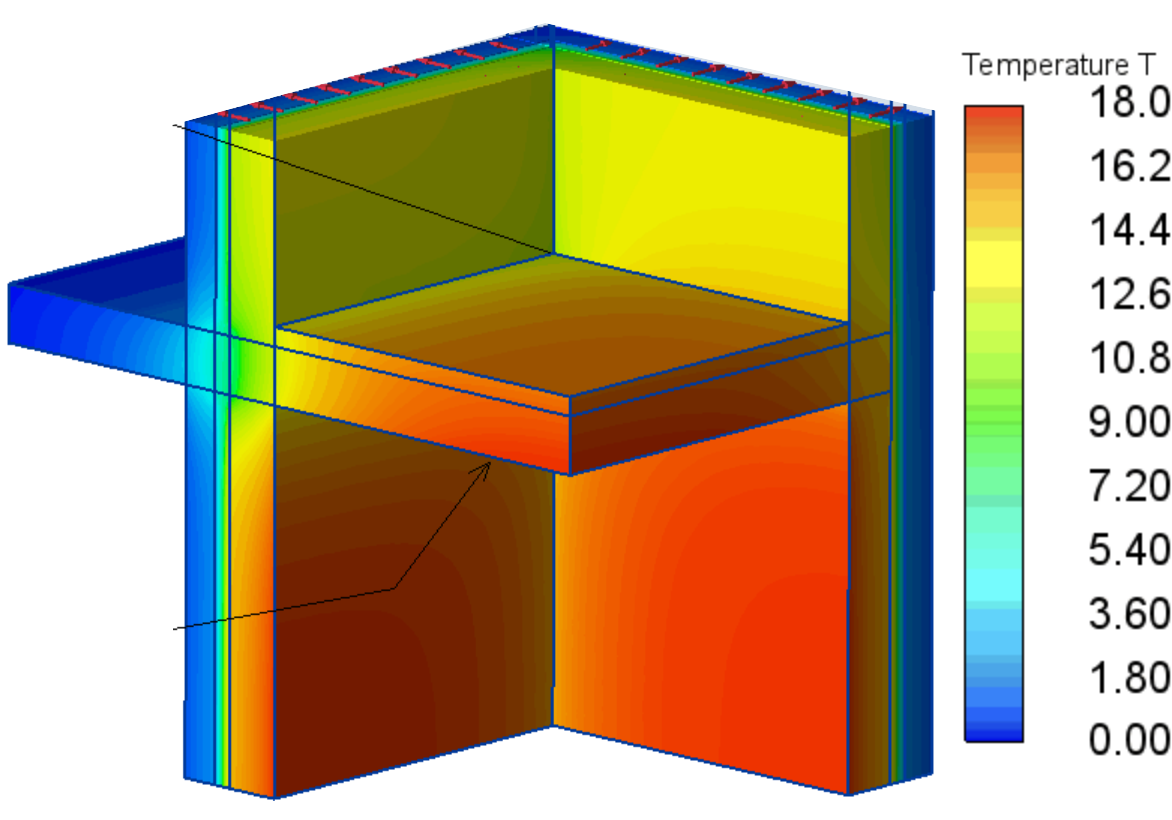
\includegraphics[width=0.65\columnwidth]{Figures/ValidationCaseClean.png}


    %\hspace{3.5cm}\textbf{a}\hfill\textbf{b}\hspace{3.5cm}
    
     \textbf{c}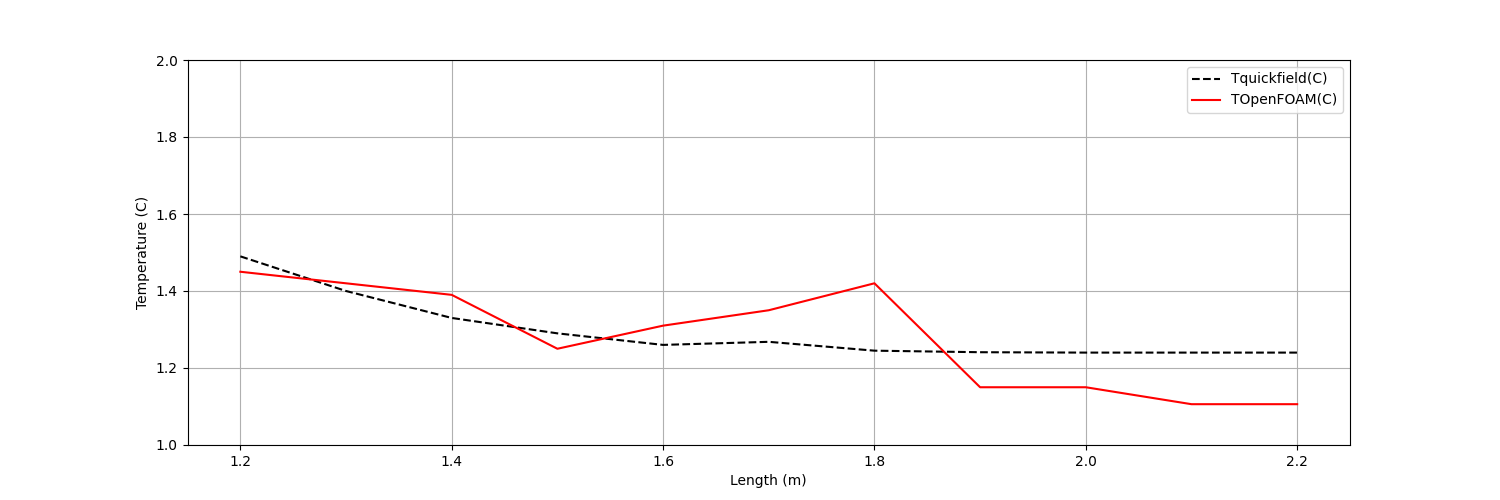
\includegraphics[width=1\columnwidth, clip = true]{Figures/Figure_2.png}
    \caption[3D Validation Plots]{Validation Plots. \textbf{(a)} \textbf{(b)}  \textbf{(c)} }
    \label{fig:validation-plots}
\end{figure}
\todo{Remove (c) from this figure and put it in separate figure. }






\section{Discussion}

The results illustrate the capabilities of using Rhinoceros and Grasshopper to simplify the pre-processing and post-processing steps to run the 3D heat transfer simulation in OpenFOAM. The simulation focuses on convective and conductive heat transfer for a 3D heat transfer problem. 
\todo{describe case study. It is a corner section of a building with a balcony}
In some cases running the solver results in a diving by zero error which is SIFPE, but, the Grasshopper script needs to be recomputed due to opening a new Rhino file or making changes in the text files in the case path. 
\todo{don't just say that! describe where the error exactly comes from!!! just saying some cases, doesn't help anyone. }

The experimental design section can be easily validated by setting up a transient heat transfer case using the same \textit{chtMultiRegionFoam}. However, due to time constraints, three timesteps were chosen from the experimental results to be simulated in three separate steady-state heat transfer cases. The results are shown in \ref{table2d}, \ref{error2d} and \ref{fig:expr}. 
\todo{start by saying what you have done, then say what more you could have done. say the CHT solver has transient capabilities and that you can provide time-dependent boundary conditions to leverage that capability.}

Additional potential to the simulation is enabling the users to visualize the thermal comfort in the space (temperature of fluid in the space). Also, the use of the adaptable \textit{chtMultiRegionFoam} solver is designed to simulate complex heat transfer scenarios for various applications. It is suitable for analyzing and helping model the performance of heating and cooling systems in the HVAC  industry. The automotive industry also uses the solver to better understand engine cooling. Other uses for this solver include evaluating solar heat gain and analyzing heat exchangers.
\todo{dont talk about automotive here, just focus on how you could use your workflow and improved versions of it for buildings}

Using \textit{QuickField} to post-process the validation case presents several shortcomings when compared to the OF simulation shown in this paper. These limitations include the inability to customize the probing locations, limited visualization capabilities, and the absence of point density adjustment in the temperature plots. These constraints affect and limit us to compare specific temperature plots. 
Also, the limitations impacted the accuracy and flexibility of the 3D heat transfer simulations conducted by \textit{QuickField}. \todo{I do not understand that.}

The workflow presented in the paper is an extension of the work on 2D conductive heat transfer using OF in Solving Thermal Bridging Problems for Architectural Applications with OpenFOAM by \cite{kastner2020solving}.  \todo{sounds like you should start with this sentence. Did you look at my research seminar materials that I sent you?!}
The findings highlight several issues in the field, such as cost-effective software, and disconnection between architectural modeling software with heat transfer software. Finally, the simulation is currently automated, but the goal is to provide it as a plug-in tool in \textit{Grasshopper}.

